\documentclass[a4paper]{report}

% Polish letters packages (for OS X)
\usepackage[utf8]{inputenc}
\usepackage{polski}
\usepackage[polish]{babel}

\usepackage[T1]{fontenc}
\usepackage{textcomp}
\usepackage{lmodern}
\usepackage[a4paper, margin=1in]{geometry}
% do robienia tabel które mieszczą się na stronie (łamanie linii w kolumnach tabeli)
\usepackage{tabulary}
% do wrzucania obrazów
\usepackage{graphicx}
\usepackage{float}
% scieżka do folderu z plikami graficznymi
\graphicspath{{./images/}}
% do opisu tabel i rysunków
\usepackage{caption}
\captionsetup[table]{name=Tabela}
% do tabel żeby robić kreski (toprule, bottomrule itp)
\usepackage{booktabs}
% do kolorowania wierszy w tabeli
\usepackage{color, colortbl}
\definecolor{Gray}{gray}{0.75}
% do tworzenia własnych styli formatowania komórek tabel
\usepackage{array}
\newcolumntype{X}[1]{>{\raggedright\let\newline\\\arraybackslash\hspace{0pt}}m{#1}}
% do schowania napisu rozdzial n
\usepackage{titlesec} 
\titleformat{\chapter}[display]{\normalfont\bfseries}{}{0pt}{\Huge}
% do dodawania listingów kodu
\usepackage{listings}
% obracanie strony do landsacape
\usepackage{pdflscape}

\title{\huge Układy Cyfrowe i Systemy Wbudowane 2\\Projekt Synthesia}
\date{} % pusta data
\author{Jan Luch\hspace{42pt} 218150  \\Dawid Aksamski\hspace{5pt} 218429}


\begin{document}

\frenchspacing
\pagenumbering{gobble}
\maketitle
\newpage

\tableofcontents
\newpage

\pagenumbering{arabic}

\chapter{Wstęp}
	\section{Cel i zakres}
	\section{Sprzęt}
	\section{Protokoły}
	\section{Interfejsy}
	\section{Algorytmy}

\chapter{Projekt}
	\section{Hierarchia}
	Krótka proza
		\subsection{Schemat}
		\subsection{Submoduły}
\chapter{Moduły}
	\section{Generator Dźwięku}
		\subsection{Symbol}
			\begin{figure}[h!]
				\centering
				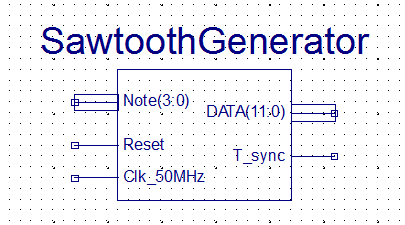
\includegraphics{sawtoothgenerator2.png}
				\caption{Moduł generujący falę piłokształtną}
			\end{figure}
		\subsection{Porty}
		{\Large Wejścia:}
			\begin{itemize}	 
				\item \textbf{Note} - wektor w zakresie od 0 do 13 odpowiadający za wysokość generowanego dźwięku
				\item \textbf{Reset} - resetowanie procesu generowania fali piłokształtnej
				\item \textbf{Clk\_50MHz} - sygnał zegarowy
			\end{itemize}
		{\Large Wyjścia:}
			\begin{itemize} 
				\item \textbf{DATA} - wektor w zakresie od 0 do 4032 przesylany do modułu DAC\_Write
				\item \textbf{T\_sync} - sygnał startu przesyłania
			\end{itemize}
		\subsection{Najważniejsze sygnały i procesy}
		{\Large Sygnały:}
			\begin{itemize}
				\item \textbf{counter} - licznik pojedynczego przebiegu fali (jeden \"ząb\" piły
				\item \textbf{tickCounter} - lcznik dzielący częstotliwość wejściową
				\item \textbf{ts} - sygnał startu przesyłania
				\item \textbf{index} - numer elementu tablicy zawierającej granice licznika dla poszczególnych częstotliwości dźwięku
				\item \textbf{pitch} - tablica typu \textbf{notes} zawierająca granice licznika dla dźwięków od C4 do C5 dla systemu równomiernie temperowanego, A4 = 440Hz
			\end{itemize}
		{\Large Procesy:}
			\begin{itemize}
			\item Proces odpowiedzialny za licznik dzielący częstotliwość oraz za generowanie sygnału startu przesyłania\\
				\lstinputlisting[language=VHDL, firstline=83, lastline=97,frame=single,tabsize=2]{SawtoothGenerator.vhd}
			\item Proces odpowiedzialny za licznik pojedynczego przebiegu fali\\
				\lstinputlisting[language=VHDL, firstline=100, lastline=111,frame=single,tabsize=2]{SawtoothGenerator.vhd}
			\item Proces odpowiedzialny za zwrócenie wektora wyjściowego na najstarszych bitach, ze względu na moduł DAC\_Write, który odczytuje najstarsze bity\\
				\lstinputlisting[language=VHDL, firstline=117, lastline=117,frame=single,tabsize=2]{SawtoothGenerator.vhd}
			\end{itemize}
		\subsection{Symulacja}
		
		\newpage
	\section{Sterownik VGA}
		\subsection{Symbol}
			\begin{figure}[h!]
				\centering
				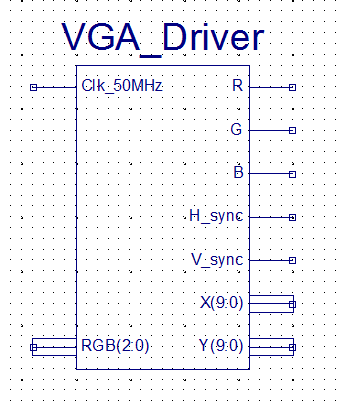
\includegraphics{vgadriver2.png}
				\caption{Moduł sterujący wyjciem VGA}
			\end{figure}
		\subsection{Porty}
		\subsection{Najważniejsze sygnały i procesy}
		\subsection{FSM}
		Graf i opis kodu
		\subsection{Symulacja}
	\newpage
	\section{Przełącznik}
		\subsection{Symbol}	
			\begin{figure}[h!]
				\centering
				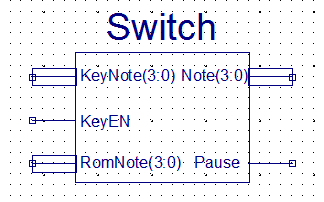
\includegraphics{switch2.png}
				\caption{Moduł Switch}
			\end{figure}
		\subsection{Porty}
			{\Large Wejścia:}
			\begin{itemize}	 
				\item \textbf{KeyNote} - wektor w zakresie od 0 do 13 odpowiadający numerowi przychodzącej nuty z modułu klawiatury
				\item \textbf{KeyEN} - ustawianie trybu w jakim ma działać urządzeni(1 - klawiatura, 0 - pozytywka)
				\item \textbf{RomNote} - wektor w zakresie od 0 do 13 odpowiadający numerowi przychodzącej nuty z modułu pozytywki
			\end{itemize}
		{\Large Wejścia:}
			\begin{itemize} 
				\item \textbf{Note} - wektor w zakresie od 0 do 13 ustawiany w zależności od trybu w jakim pracuje urządzenie
				\item \textbf{Pause} - sygnał zatrzymujący animację pozytywki
			\end{itemize}
		\subsection{Najważniejsze sygnały i procesy}
			{\Large Procesy:}
				\begin{itemize}
					\item Proces odpowiedzialny za ustawianie wektora wyjściowego Note w zależności od sygnału KeyEN\\
						\lstinputlisting[language=VHDL, firstline=43, lastline=43,frame=single,tabsize=2]{Switch.vhd}
					\item Proces odpowiedzialny za ustawianie synału pauzy w zależności od sygnału KeyEN\\
						\lstinputlisting[language=VHDL, firstline=44, lastline=44,frame=single,tabsize=2]{Switch.vhd}
				\end{itemize}
	
		\begin{landscape}
			\subsection{Symulacja}
				\begin{figure}[h!]
					\centering
					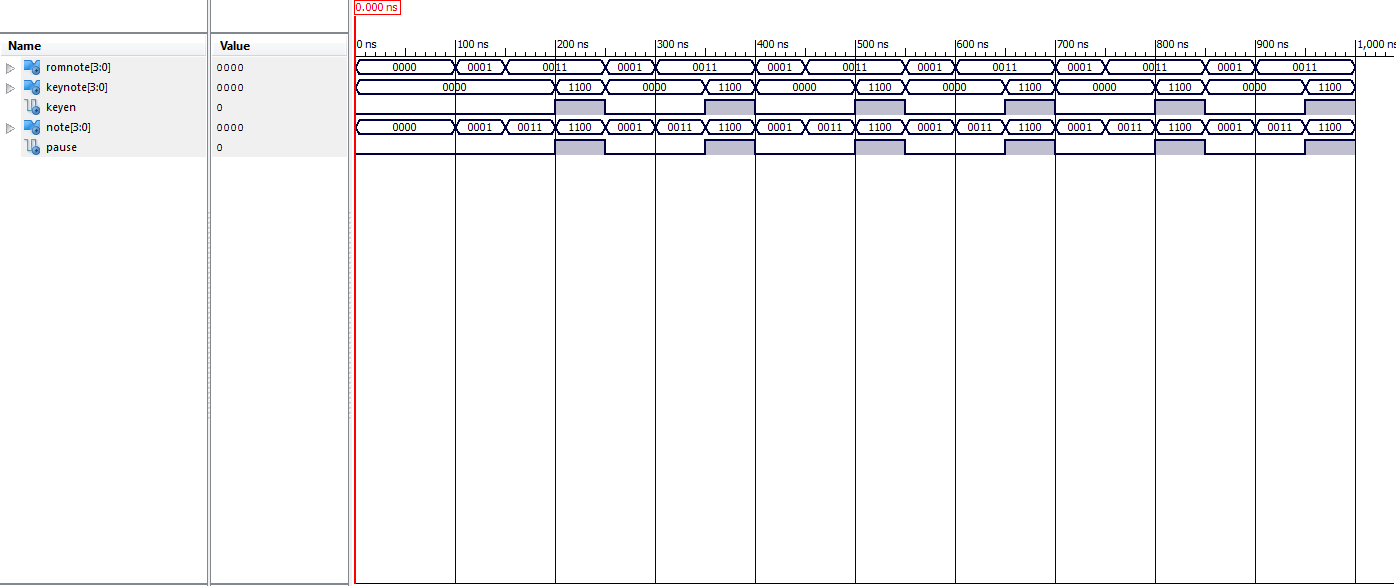
\includegraphics[width=1.6\textwidth]{switch_symulacja2.png}
					\caption{Sumulacja modeułu Switch}
				\end{figure}
		\end{landscape}
			Na symulacji widać zmianę
	\section{Czytnik kodów z klawiatury}
		\subsection{Symbol}
			\begin{figure}[h!]
				\centering				
				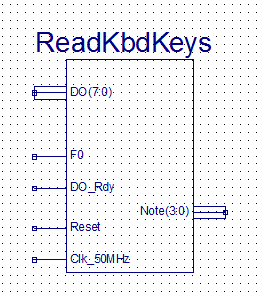
\includegraphics{readkbdkeys2.png}
				\caption{Moduł czytający kody z klawiatury}
			\end{figure}
		\subsection{Porty}
			\lstinputlisting[language=VHDL, firstline=4, lastline=11,frame=single]{ReadKbdKeys.vhd}
		\subsection{Najważniejsze sygnały i procesy}
		\subsection{FSM}
		Graf i opis kodu
		\subsection{Symulacja}
		\newpage
	\section{Synthesia}
		\subsection{Symbol}
			\begin{figure}[h!]
				\centering
				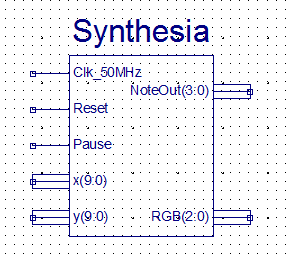
\includegraphics{synthesia2.png}
				\caption{Moduł zarządzający wyświetlaniem animacji oraz generowaniem melodii}
			\end{figure}
		\subsection{Porty}
		{\Large Wejścia:}
			\begin{itemize}	 
				\item	\textbf{Clk\_50MHz} - sygnał zegarowy
				\item \textbf{Reset} - resetowanie pracy modułu
				\item 	\textbf{Pause} - wstrzymywanie wyświetlania animacji
				\item \textbf{X, Y} - współrzędne aktualnie rysowanego punktu na ekranie
			\end{itemize}
		{\Large Wyjścia:}
			\begin{itemize} 
				\item 	\textbf{NoteOut} - wektor w zakresie od 0 do 13 odpowiadający za wysokość dźwięku do odtworzenia
				\item 	\textbf{RGB} - wektor w zakresie od 0 do 7 odpowiadający za wyświetlany kolor
			\end{itemize}
		\subsection{Najważniejsze sygnały i procesy}
		{\Large Sygnały:}
			\begin{itemize}
				\item \textbf{key\_position} - tablica elementów typu integer, przechowujących wartości pozycji horyzontalnej kolejnych dźwięków
				\item \textbf{should\_play} - sygnał typu STD\_LOGIC, przechowujący informację o tym, czy należy odtwarzać melodię z syntezatora
				\item \textbf{keys\_to\_display} - tablica elementów typu note - tablica 3 integerów - przechowujących kolejno: numer nuty, pozycję wertykalną graficznej reprezentacji dźwięku, wysokość graficznej reprezentacji dźwięku, jednocześnie odpowiadającą długości jego trwania
			\end{itemize}
		{\Large Procesy:}
			\begin{itemize}
			\item Proces odpowiedzialny rysowanie graficznej reprezentacji dźwięków na ekranie\\
						\lstinputlisting[language=VHDL, firstline=134, lastline=180,frame=single,tabsize=2]{Synthesia.vhd}
			\item Proces odpowiedzialny za animowanie graficznej reprezentacji melodii\\
									\lstinputlisting[language=VHDL, firstline=182, lastline=194,frame=single,tabsize=2]{Synthesia.vhd}
			\item Proces odpowiedzialny za wybranie odpowiedniego dźwięku do odtworzenia na podstawie animacji\\
									\lstinputlisting[language=VHDL, firstline=196, lastline=257,frame=single,tabsize=2]{Synthesia.vhd}
			\end{itemize}
	
		\subsection{Symulacja}
	
\chapter{Implementacja}
	\section{Rozmiar}
	LUT, BRAM
	\section{fmax}
	\section{Podręcznik użytkowania urządzenia}
	(Zdjęcia)
	
\chapter{Podsumowanie}
	\section{Ocena krytyczna}	
	\section{Kierunki dalszych prac}
	
\chapter{Literatura}

\begin{figure}
	\caption{Sample figure}
\end{figure}
		
\begin{table}
	\caption{Sample table}
\end{table}

% Compile twice to generate list of tables and figures properly
\begin{appendix}
	\listoffigures
	\listoftables
\end{appendix}



\end{document}
